\section{Evaluation}
\label{sec:evaluation}

To be able to compare the results of different experiments, we have fixed the number of iterations of Stochastic Gradient Descent to a constant value of $20000$.

\subsection{Train Error}
\begin{figure}[t]
	\centering
	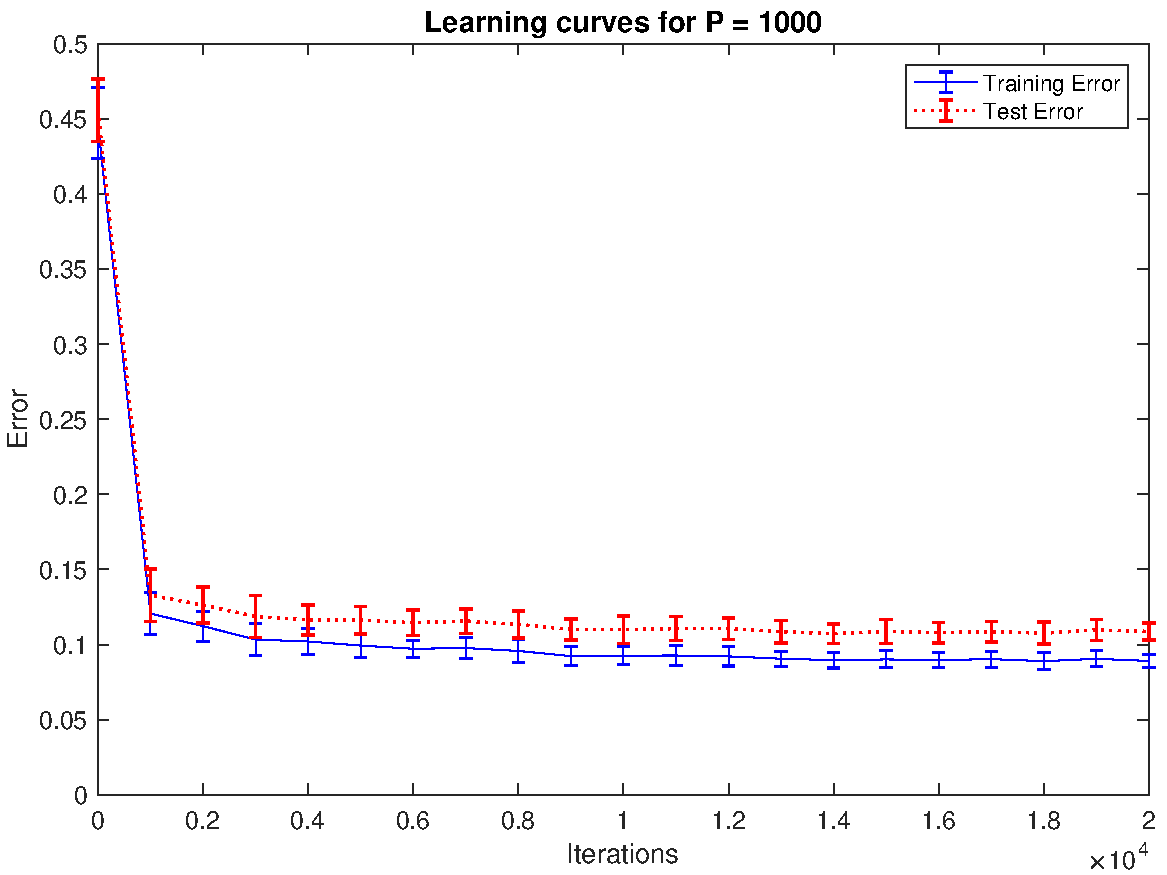
\includegraphics[width=\columnwidth]{figures/error}
	\caption{Train and test error of the network for $P = 1000$. Training executed with a fixed
	learning rate $\eta = 0.05$.}
	\label{fig:training_error}
\end{figure}

\cref{fig:training_error} shows the train and test error for the network trained using Stochastic Gradient Descent on the first $1000$ examples.
Both the train error and test error drop very quickly during approximately the first $1000$ iterations, then remain almost constant for the rest of the training.
The test error is slightly bigger than the train error:
at the end of the training, the train error is around $0.10$ and the test error around $0.12$.
Since the test error never increases, the model does not seem to overfit the training data.

\subsection{Learned Weights}
\begin{figure}[t]
	\centering
	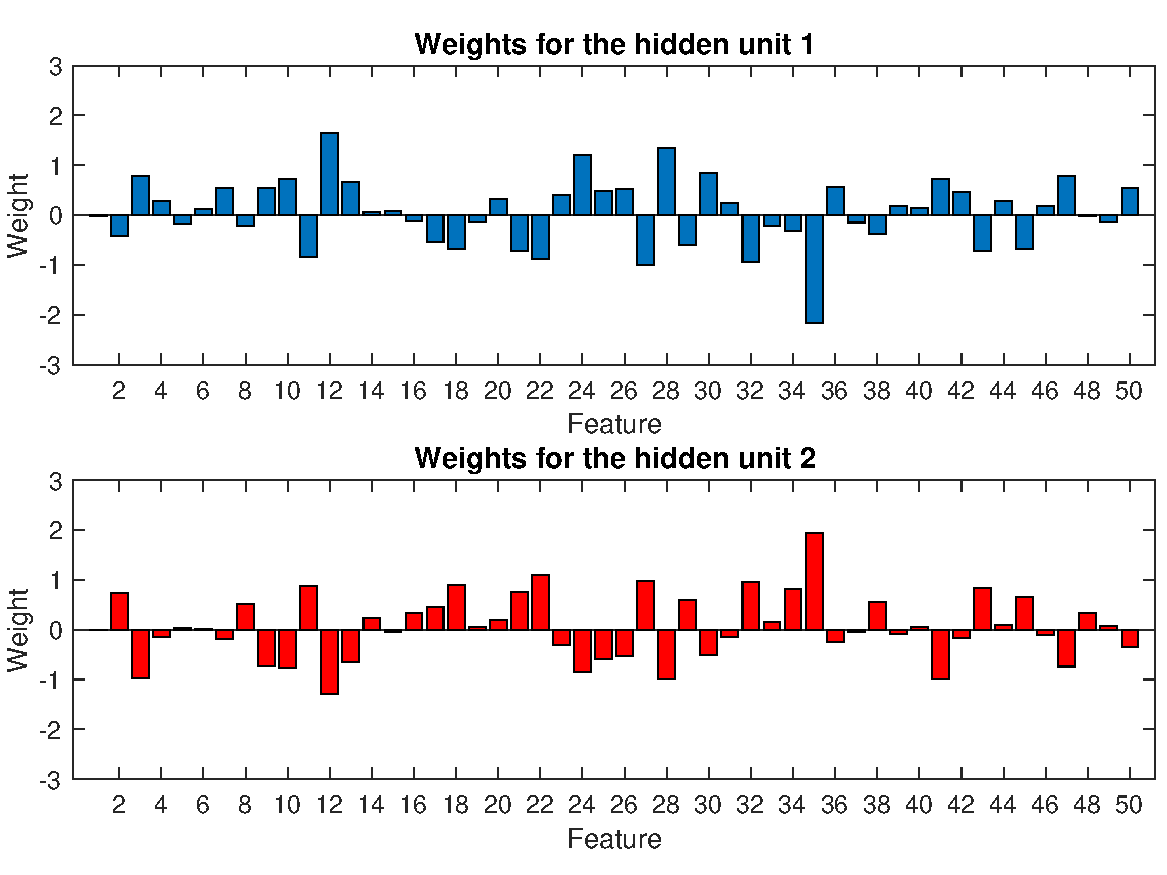
\includegraphics[width=\columnwidth]{figures/weights_p_1000}
    \caption{Weights of the hidden units of the network after the training.}
	\label{fig:weights}
\end{figure}

\cref{fig:weights} shows the weights learned from the hidden units of the networks after the training for $P = 1000$.
As expected, the units learn different weights thanks to the random initialization of the weights.

\subsection{Train Dataset}
\begin{figure}[t]
	\centering
	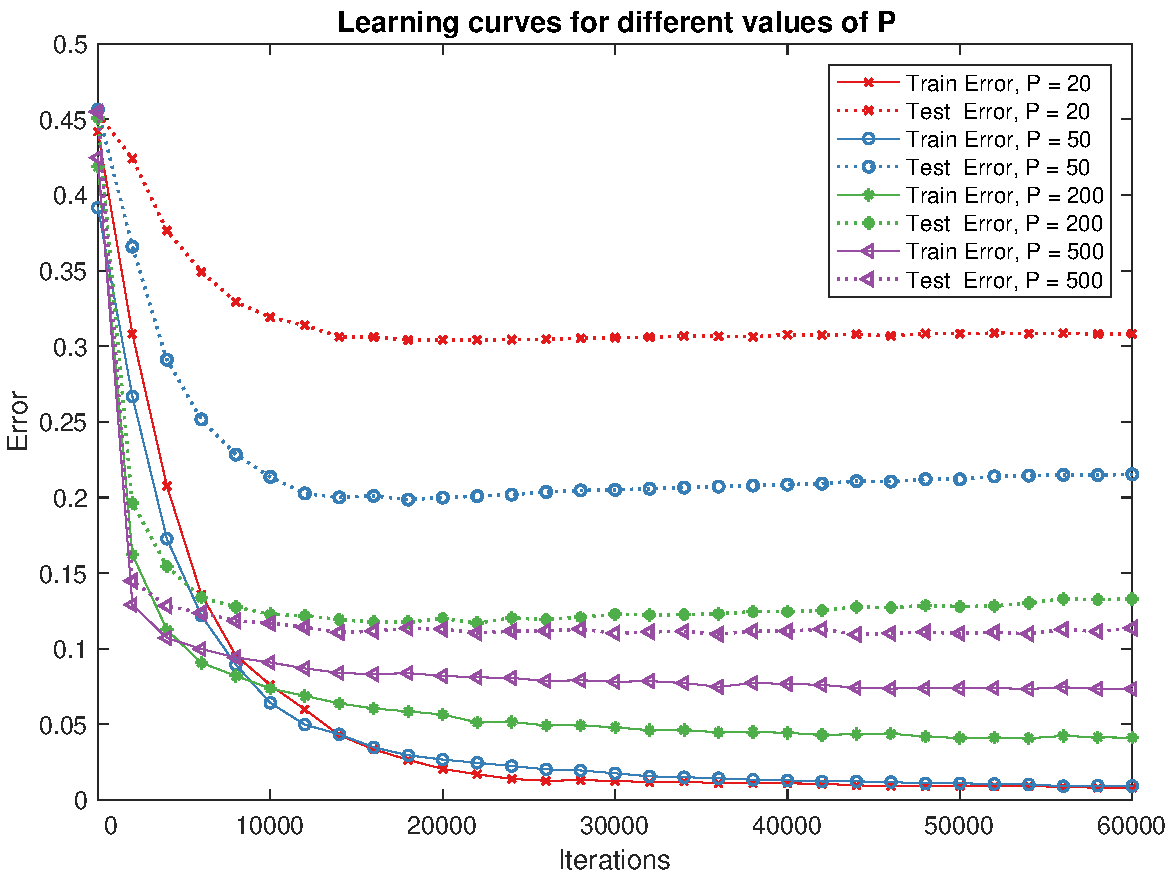
\includegraphics[width=\columnwidth]{figures/error_ps}
	\caption{Train and test error of the network for different numbers of training examples $P$. Trainings
	executed with a fixed learning rate $\eta = 0.05$.}
	\label{fig:ps}
\end{figure}

\cref{fig:ps} shows the train and test error for different values of $P$, i.e. for a network trained on training dataset of different dimensions.
For very small training datasets ($P = 20$, $P = 50$), the train error drops very quickly and stabilizes close to $0$;
the test error is high and even increases during the training for $P = 50$.
It seems like the network does not see enough examples to generalize properly to new data and tends to overfit the train set.

For $P = 200$, the train error is higher, but the test error gets significantly smaller.
Still, the test error increases during the training, which indicates overfit.

For $P = 500$, the train and test error get closer and remain constant during most of the training.
The results for higher values of $P$ are really similar and are thus not shown.

\subsection{Train Policy}
The learning rate is well known to influence the number of iterations the network needs to minimize
its cost function. It is nevertheless true that a high value for this variable causes the network to
be unstable since it learns the same amount of information from all the data that are presented to it (no matters the number of iterations).
For this reason we decided to implement some different schedulers for the learning rate able to change its
value over time as a function of the iterations.

The implemented learning rate policies (LRPs) are: \textit{fixed}, \textit{step}, \textit{exponential} and \textit{cycle}.
In the figure below \cref{fig:learning_rates_policies} it's possible to take a look at the way they change the value of the learning rate over time,
or better saying over the iterations.

\begin{figure}
	\centering
	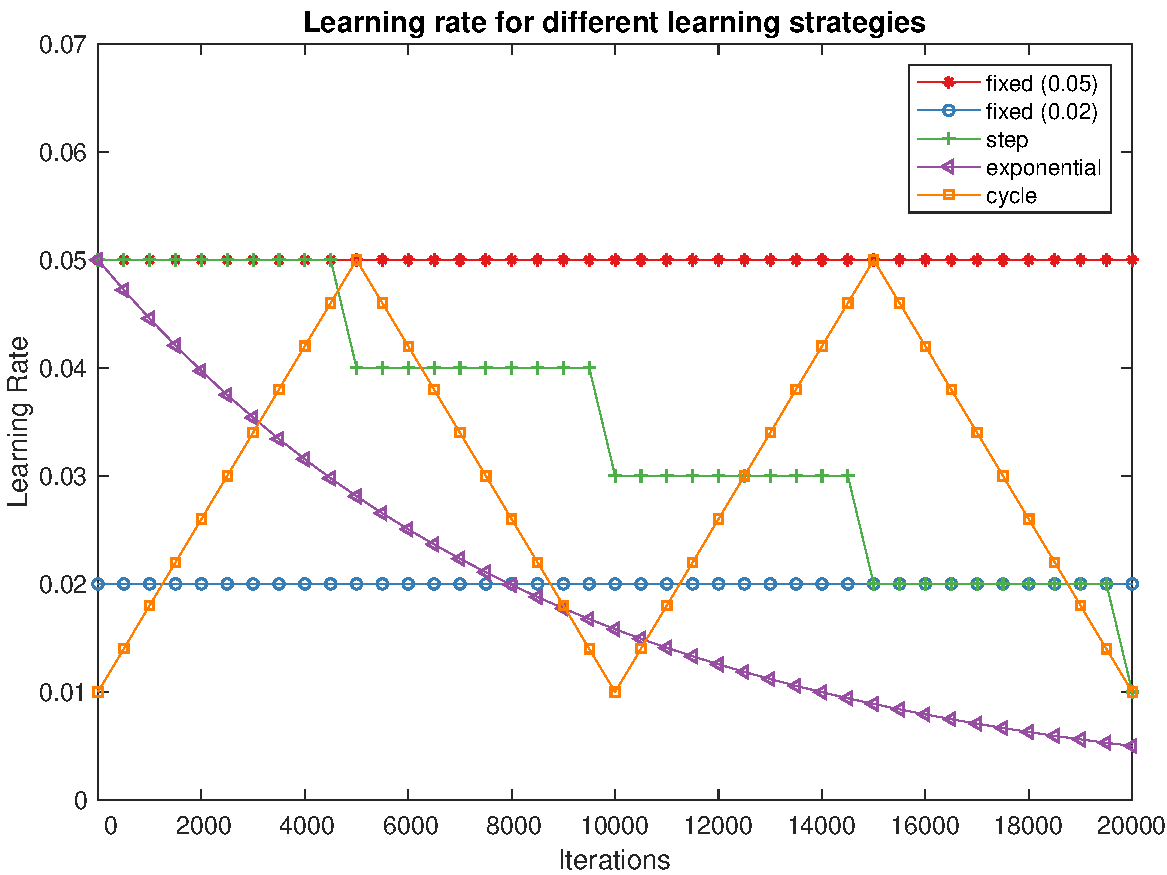
\includegraphics[width=\columnwidth]{figures/learning_rates}
	\caption{Learning rate evolution over iterations for different learning rate policies.}
	\label{fig:learning_rates_policies}
\end{figure}

From the application of these learning rates we expect a change in the behavior of the error function. In particular
since we are decreasing the learning rate from an iteration to the other we expect the error to be more stable (exception made
for what concerns the \textit{cycle} LRP).

As it is possible to see in \cref{fig:lrp_training_error} the different LRPs have different
effects on the error and we are going to explain it more in details from case to case.

\begin{figure}
	\centering
	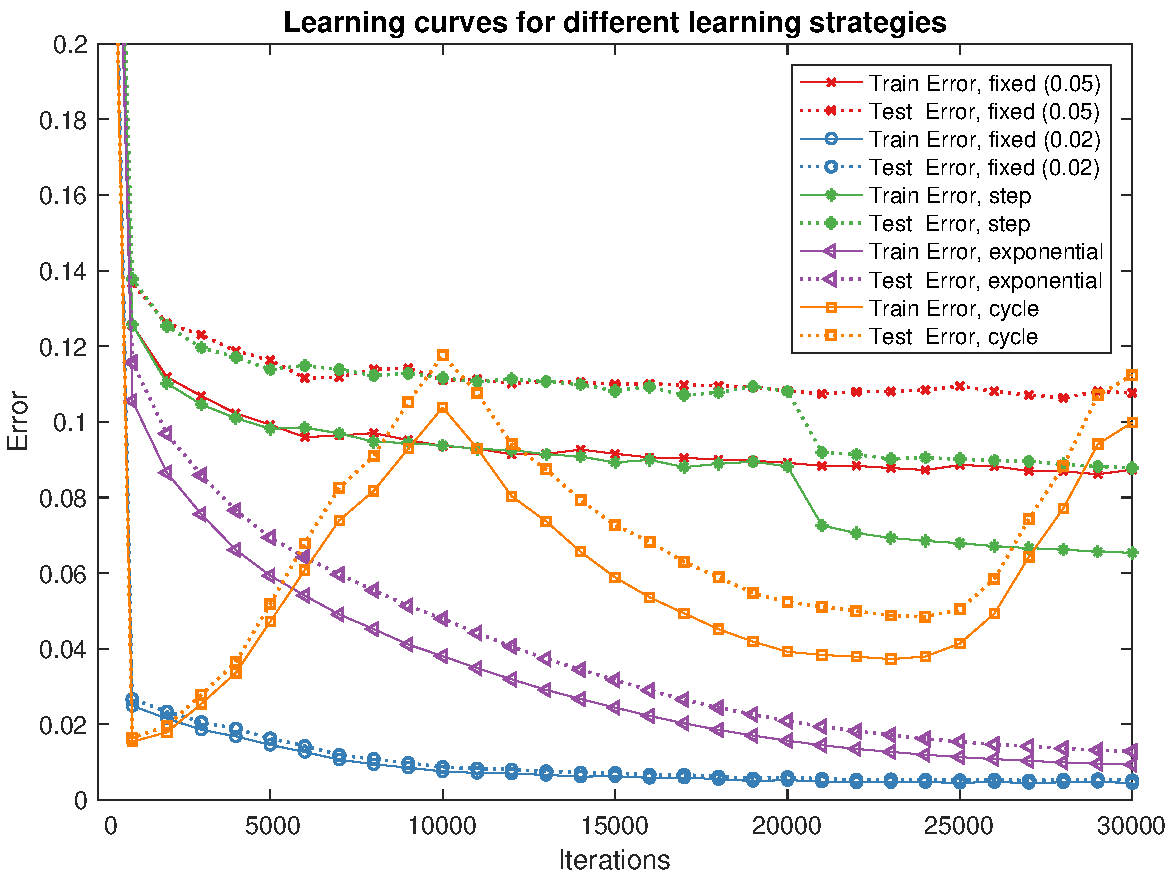
\includegraphics[width=\columnwidth]{figures/error_strategies.pdf}
	\caption{Training and test error for different learning rate policies.}
	\label{fig:lrp_training_error}
\end{figure}

\subsubsection{Fixed LRP}
As the name suggests this LRP leaves the learning rate fixed during iterations. We can notice the error to drop down after around 500 iterations and then
to remain pretty stable and to maintain a tendency to decrease slowly, meaning that the network learned most
of the information from the data. With this data this LRP also seems to be the best performing one when a learning rate of $\eta = 0.02$ is chosen.

\subsubsection{Step LRP}
This LRP consists in decreasing the learning rate of a defined quantity (\textit{drop}) after a certain number of iterations
(\textit{stepsize}). In \cref{fig:learning_rates_policies} it's possible to notice that the steps happen exactly after 5'000 iterations and that
the learning rate is reduced of $0.01$ each time.
The decrement in the value of the learning rate mirrors in a some error's drops just after its update as it's possible to see in \cref{fig:lrp_training_error}.

\subsubsection{Exponential LRP}
This LRP consist in decreasing the learning rate in an exponential way (i.e. dividing it by a constant value over the iterations). This
LRP lets the network learn quickly in the beginning, when the weights are still far from the teacher, and slowly while they're getting closer. The plot
relative to this LRP in \cref{fig:lrp_training_error} shows a smoother decrease of the error which just after 3'000 iterations tends to have a value
smaller than $0.01\%$.

\subsubsection{Cycle}
This LRP consists in increasing and decreasing the learning rate linearly over the number of iterations creating a sawteeth plot as it's noticeable
in \cref{fig:learning_rates_policies}. The aim of this LRP is to avoid local minima letting the value of the learning rate to grow again after it
reached it's minimum value. As it's possible to see in \cref{fig:lrp_training_error} with the data provided the LRP performs well as far
as the value of the learning rate is smaller than the \textit{fixed}($0.02$) one and then the error increases following the increase of the learning rate and never
goes back to its early low value.

Overall it's to notice that all the implemented LRPs perform better than the \textit{fixed}($0.05$), as it was expected in the introduction of this section.